% ОБЯЗАТЕЛЬНО ИМЕННО ТАКОЙ documentclass!
% (Основной кегль = 14pt, поэтому необходим extsizes)
% Формат, разумеется, А4
% article потому что стандарт не подразумевает разделов
% Глава = section, Параграф = subsection
% (понятия "глава" и "параграф" из стандарта)
\documentclass[a4paper,article,14pt]{extarticle}

% Подключаем главный пакет со всем необходимым
\usepackage{spbudiploma}

% Пакеты по желанию (самые распространенные)
% Хитрые мат. символы
\usepackage{euscript}
% Таблицы
\usepackage{longtable}
\usepackage{makecell}
% Картинки (можно встявлять даже pdf)
\usepackage[pdftex]{graphicx}

\usepackage{amsthm,amssymb, amsmath}
\usepackage{textcomp}


\begin{document}

% Титульник в файле titlepage.tex
% --------------------- Стандарт СПбГУ для ВКР --------------------------
% Автор: Тоскин Николай, itonik@me.com
% Если заметили ошибку, напишите на email
% Если хотите добавить изменение самостоятельно, GitHub: . PR-s welcome!
% Использованы материалы:
% habr.com/ru/post/144648/
% cpsconf.ru
% Текст:
% http://edu.spbu.ru/images/data/normativ_acts/local/20181030_10432_1.pdf
% Титульный лист:
% http://edu.spbu.ru/images/data/normativ_acts/local/20180703_6616_1.pdf
% -----------------------------------------------------------------------

% Титульный лист диплома СПбГУ
% Временное удаление foot на titlepage
\newgeometry{left=30mm, top=20mm, right=15mm, bottom=20mm, nohead, nofoot}
\begin{titlepage}
\begin{center}
% Первый символ съедается, первым знаком поставлен Ы
\textbf{Санкт--Петербургский}
\textbf{государственный университет}

\vspace{35mm}

\textbf{\textit{\large КОВАЛЕНКО Лев Алексеевич}} \\[8mm]
% Название
\textbf{\large Выпускная квалификационная работа}\\[3mm]
\textbf{\textit{\large Детектирование и классификация дефектов 
нефтепроводов на основе данных 
внутретрубных роботов-дефектоскопов}}

\vspace{20mm}
% Булшит
Уровень образования: бакалавриат\\
Направление 01.03.02 «Прикладная математика и информатика»\\
Основная образовательная программа СВ.5005.2016
«Прикладная математика, фундаментальная информатика и программирование»\\
Профиль «Математическое и программное обеспечение \\ вычислительных машин»\\[30mm]


% Научный руководитель, рецензент
% Сходить в уч отдел и узнать, правильно ли
\begin{flushright}
{Научный руководитель:} \\
доцент, кафедра технологии программирования, \\ к.т.н.  Блеканов~Иван Станиславович
\end{flushright}
\begin{flushright}
{Рецензент:} \\
ООО ИТСК, \\  Кононов~Ярослав Сергеевич
\end{flushright}

\vfill 

{Санкт-Петербург}
\par{2020 г.}
\end{center}
\end{titlepage}
% Возвращаем настройки geometry обратно (то, что объявлено в преамбуле)
\restoregeometry
% Добавляем 1 к счетчику страниц ПОСЛЕ titlepage, чтобы исключить 
% влияние titlepage environment
\addtocounter{page}{1}

% Содержание
\tableofcontents
\pagebreak

\specialsection{Введение}
В промышленности на сегодняшний день появилось огромное количество программных комплексов и 
информационных систем позволяющих автоматизировать и оптимизировать производство. 
Такая тенденция подталкивает различные промышленные компании к внедрению инноваций 
в технологические процессы и проведение различных исследований. 

Большой толчок в развитии получили многие области промышленности, например автомобильная промышленность или нефтегазовая. 
Примером этому может служить то, что за последние несколько лет в группе компаний Газпром Нефть были 
внедрены инновационные решения для оптимизации процессов \cite{j1}:
\begin{itemize}
    \item Инструмент для планирование очистки призабойной зоны для увеличения точности прогнозирования ожидаемого эффекта.
    \item Проект “Умная логистика” позволяет оптимизировать логистику поставки нефти и упростить контроль.
    \item Информационной система «ЭКСПРЕСС-ОЦЕНКА ГЕОЛОГИЧЕСКОГО СТРОЕНИЯ И ВЕРИФИКАЦИЯ ДАННЫХ», 
    автоматизирующая процесс оценки геологического строения и верификации данных, построение карт, 
    таблиц, схем геологических характеристик активов компании \cite{s1}. 	
\end{itemize}

Кроме внедрения крупных проектов, стоит отметить рост количества научно-исследовательских и опытно-конструкторских работ. 
С 2016 по 2018 их количество увеличилось в 24 раза. Исследования в компании 
Газпом Нефть проводятся по 14 различным направлениям \cite{j2}.

Одним из важных направлений для автоматизации является оценка состояния нефтепроводов \cite{a1}.
В группе компаний Газпром Нефть эксплуатируются примерно 12 тыс. км промысловых трубопроводов. В ходе эксплуатации нефтепроводы неизбежно изнашиваются. 
Это приводит к прорывам и утечкам нефти, что вызывает отрицательные экономический, экологический и репутационный эффекты. 
Во избежание этого проводятся работы по внутритрубной диагностике - съемке магнитограмм, на основе которых эксперты могут оценить состояние нефтепровода. 
Следующим этапом по развитию этого направления является автоматизация процесса оценки состояния трубопровода 
с целью уменьшения затрат по временным ресурсам и увеличению качества процесса

Практическая значимость заключается в том, что полученный в ходе работы программный комплекс может быть 
использован на предприятии для оптимизации процессов ВТД. 

На данный момент промежуток времени от проведения съемки магнитограммы до получения отчета составляет 
до 1 месяца на 10 км трубы. Использование данного инструмента в его текущей реализации позволит частично 
автоматизировать процесс интерпретации магнитограмм. Это позволит сократить временной интервал от проведения 
съемки магнитограммы до получения отчета о качестве. При некоторой доработке и улучшении качества программного 
комплекса данный процесс может быть полностью автоматизирован.

Также стоит заметить, что, за счет сокращения времени на расшифровку магнитограмм, появиться возможность 
проводить ремонтные работы раньше, что уменьшит количество прорывов нефтепроводов.


\pagebreak
\specialsection{Постановка задачи}
Цель данной работы реализовать программный комплекс, позволяющий производить автоматическое детектирвоание и классификацию дефектов, на основе анализа снимков магнитограмм. 

Для достижения цели были поставлены следующие задачи:

\begin{itemize}
    \item Провести обзор существующих решений.
    \item Собрать и подготовить данные для дальнейших исследований: перевести магнитограммы из бинарного формата в табличный, 
    провести точную разметку на основе представленных отчетов о состоянии нефтепроводов.
    \item Рассмотреть различные подходы и методы машинного обучения для детектирования швов и дефектов на различных магнитограммах.
    \item Разработать собственный подход анализа в виде модификации и комбинаций существующих алгоритмов.
    \item Выбрать стек технологий и спроектировать архитектуру программного комплекса.
    \item Разработать программное решение позволяющее проводить оценку состояния трубопровода.
    \item Провести тестирование ПО и оценку качества разработанного подхода.
\end{itemize}

\pagebreak
\section{Обзор существующих решений и подходов в области анализа состояния инженерных сооружений.}

\subsection{Обзор технологических решений}

На сегодняшний день большое количество нефтегазовы сервисных компаний предлагает проведение диагностики состояния 
трубопровода с использованием магнитных и ультразвуковых устройств. Для проведения мониторинга состояния трубопроводов 
используются автономные зонды (Рис. ~\ref{image1}.), оборудованные профилометрами и магнитными дефектоскопами. Такой зонд обычно имеет 
цилиндрическую форму, и по его бокам через равные угловые промежутки установлены измерительные блоки. Во время сервисных 
операций автономный зонд загружается в нефтепровод, а затем перемещается внутри вместе с нефтяным потоком, попутно замеряя 
магнитную индукцию вдоль стенок трубы. Полученные данные записываются в виде магнитограммы. Для ультразвуковой диагностики зон 
оснащается другим типом датчиков основанных на принципах ультразвукового замера толщины.

\begin{figure}[ht]
    \begin{center}
    \scalebox{0.7}{
       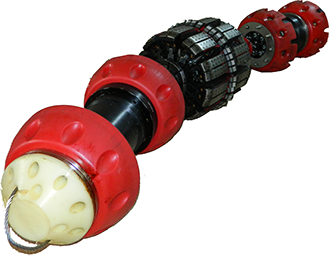
\includegraphics{images/image1.png}
    }
    
    \caption{
    \label{image1}
    Зонд для проведения внутритрубной диагностики.}
    \end {center}
\end {figure}

В сервисный компании \frqq Baker Huges\flqq предлагаются услуги по проведению магнитной и ультразвуковой внутритрубной дефектоскопии \cite{s2}.
Для провдения диагностики используются магнитный и ультрозвуковой дефектоскопы. Для интерпретации результатов дефектоскопии 
разработано ПО внутреннего пользования, позволяющее визуализировать магнитограмму и проводить ручную разметку.

Компания \frqq Интрон плюс\flqq также предлагает внутритрубную диагностику на основе данных магнитных дефектоскопов \cite{s3}. 
В компании разработано внутреннее программное обеспечение для визуализации и ручной разметки магнитограммы. 

Одним из лучших решений на рынке является решение Транснефти. У компании существует целый парк внутритрубных инспекционных 
приборов \cite{s4}. 
Магнитные дефектоскопы продемонстрированы на рисунке ~\ref{image2}.

\begin{figure}[ht]
    \begin{center}
    \scalebox{0.1}{
       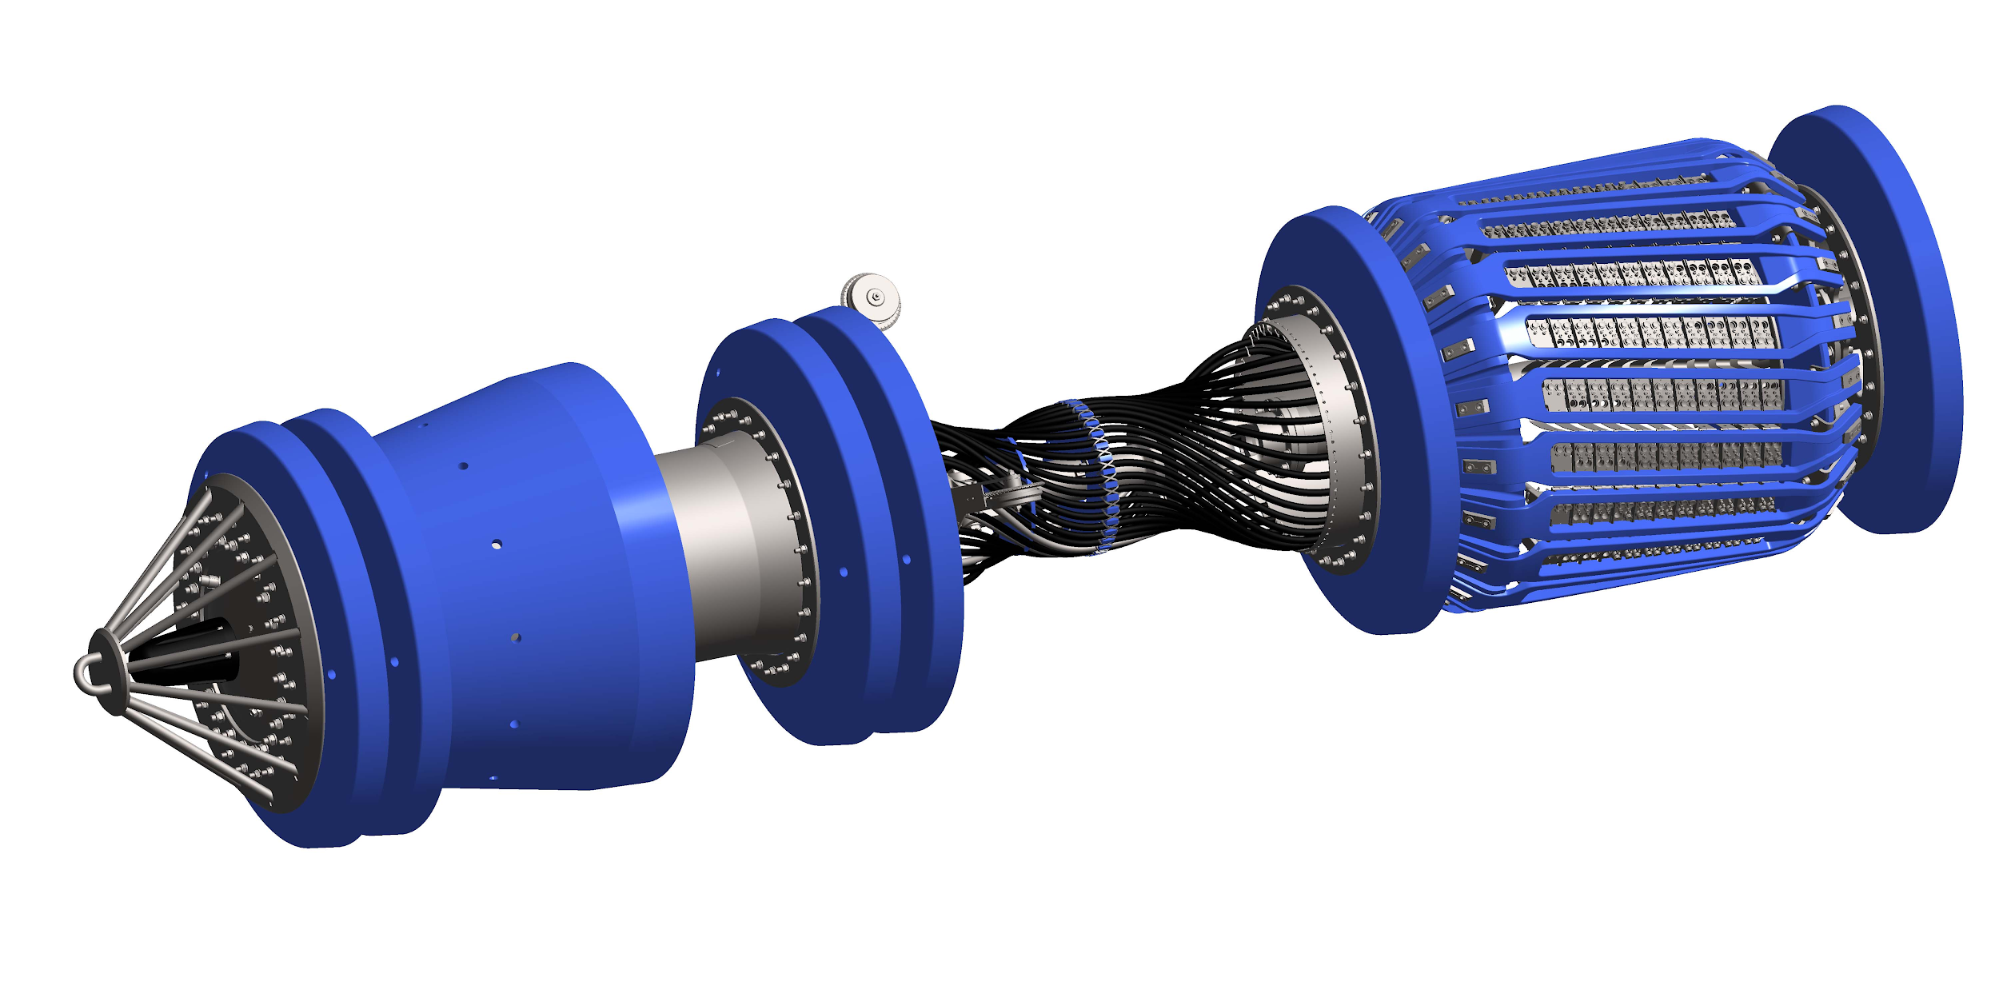
\includegraphics{images/image2.png}
       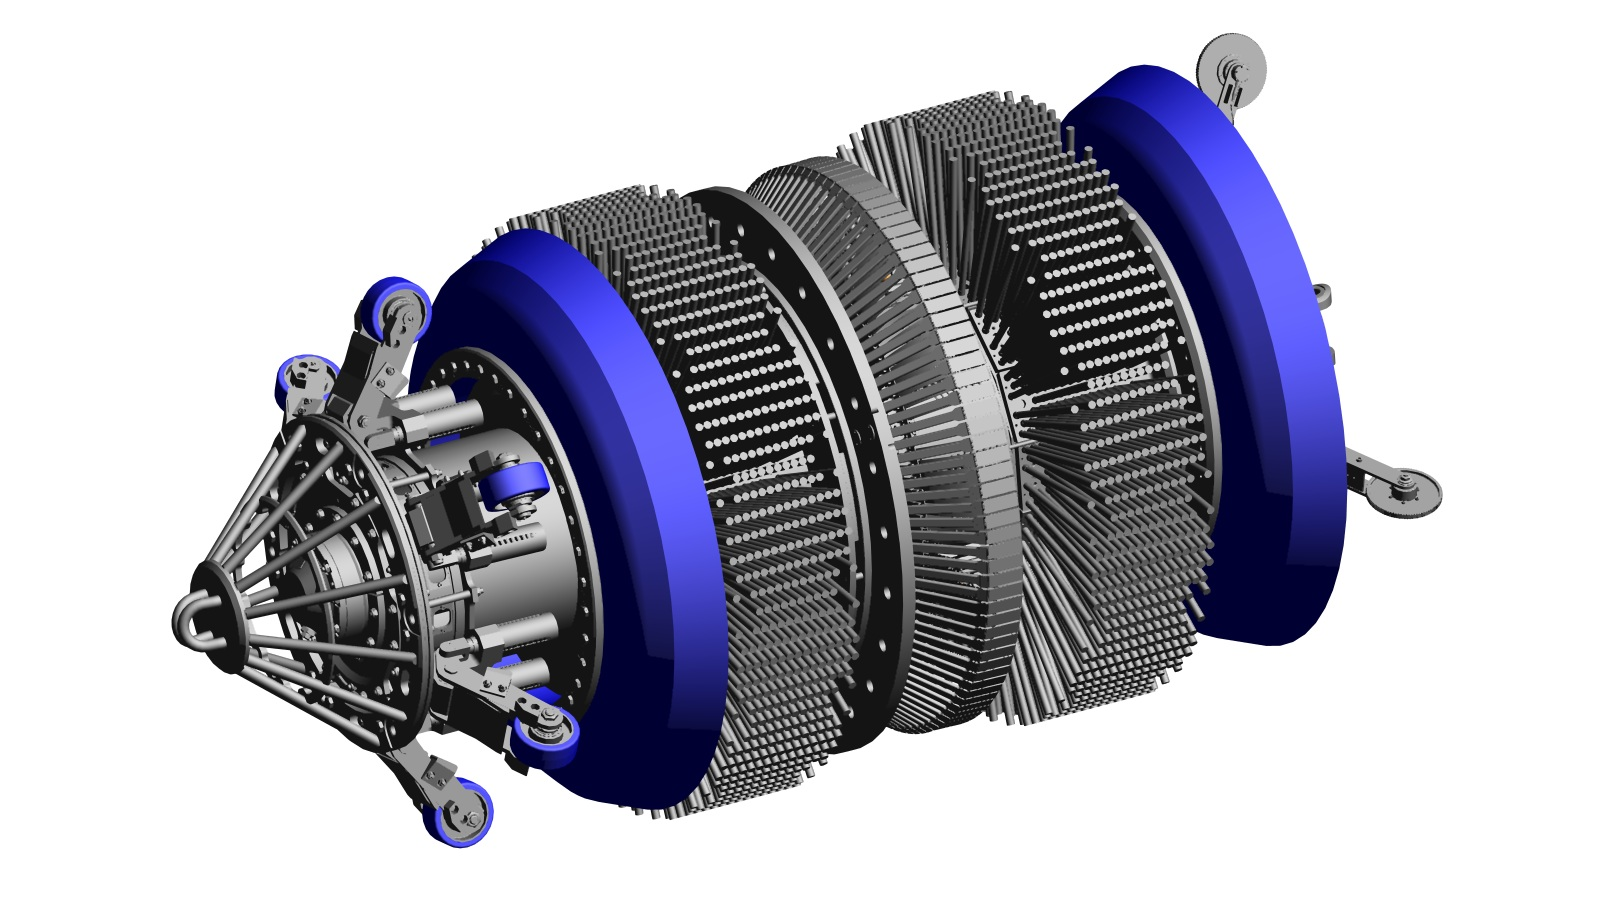
\includegraphics{images/image3.png}
    }
    
    \caption{
    \label{image2}
    Магнитные дефектоскопы.}
    \end {center}
\end {figure}

Стоит заметить что ручной анализ магнитограммы занимает длительное время, так размер одного участка трубопровода 
может составлять десятки километров. Для анализа магнитограмм такого размера у экспертов уходит более одного месяца.

Информации о существующих и эксплуатируемых программных решения для автоматизации процесса интерпретации и детектирования дефектов в открытом доступе не обнаружено.

\subsection{Обзор алгоритмов анализа данных о состоянии сети трубопроводов}

Для анализа состояния сети трубопроводов в статье \cite{a2} предлагается использовать 
статистические методы и методы машинного обучения. Сам анализ представляет собой детектирование дефектов и 
конструктивных элементов на магнитограмме, то есть классифкация участка трубы как дефект, конструктивный 
элемент или полотно трубы. Для решения этой задачи стоит в первую очередь рассмотреть алгоритмы классификации:

\begin{itemize}
    \item Random Forest Classifier – модель машинного обучения основанная на применение деревьев решений. В основе этого ансамбля лежит подход бэкинга - обучение одинаковы моделей на разных подвыборках набора данных. Он использует усреднение для повышения точности прогнозирования и контроля соответствия \cite{a3}.
    \item Extra Tree Classifier – данный алгоритм имеет такой же принцип, как и описанный выше Random Forest Classifier, но в качестве базовой модели использует рандомизированное решающее дерево \cite{a4}. 
    \item SVM Classifier – метод опорных векторов для классификации. Исходные векторы переводятся в пространство более высокой размерности, а затем в этом пространстве ищется разделяющая гиперплоскость с максимальным зазором, т.е. находящаяся максимально далеко от точек всех представленных классов \cite{a5}. 
    \item Logistic Regression - статистическая модель, позволяющая прогнозировать вероятность появление некоторого события по значениям множества признаков. Вероятность вычисляется путем сравнения события с логистической кривой \cite{a6}.
\end{itemize}

В статьях  \cite{a7}, \cite{a8} описывается использование нейронных сетей для решения подобных задач. В них фигурируют сверточные нейронные сети и сети прямого распространения.

\begin{itemize}
    \item Нейронные сети прямого распространения - многослой перцептрон, более подробно алгоритм описан в статье \cite{a9}.
    \item Сверточные нейронные сети - алгоритм на оснвое применение механизма свертки для выделения 
    признаков и дальнейшей классификации на их основе \cite{a10}.
\end{itemize}

Основываясь на природе данных - сигналы магнитометров, было принято решение рассмотреть алгоритмы  обработки сигналов, в частности алгоритмы фильтрации:

\begin{itemize}
    \item Фильтр Калмана - эффективный рекурсивный фильтр, проводит оценку вектора состояния динамической системы 
    на основе ряда неполных и зашумленных данных \cite{a11}.
    \item Вейвлет фильтр - фильтр основанный на применении вейвлет преобразования к набору сигналов \cite{a12}.
\end{itemize}

\subsection{Обзор метрик качества алгоритмов по детектированию сварных швов и дефектов}
Для оценки результатов были выбраны стандартные метрики: Recall,  Precision и F1-measure.
Эти метрики основываются на подсчете confusion matrix (матрицы ошибок), приведенной в Таблицах 1 и 2.

\begin{center}
\begin{longtable}{|p{5cm}|p{5cm}|p{6cm}|}
    \caption{Матрица ошибок для сварных швов}\\\hline
     & Сварной шов \par по разметке & Дефекты и структурные \par элементы по разметке \\ \hline
    Предсказание класса\par сварного шва & True positive & False positive \\ \hline
    Предсказание класса \par дефектов и структурных элементов & False negative & True negative \\ \hline
\end{longtable}
\end{center}

\begin{center}
\begin{longtable}{|p{5cm}|p{5cm}|p{6cm}|}
    \caption{Матрица ошибок для дефектов}\\\hline
        & Дефекты \par по разметке & Сварные швы и \par структурные элементы \par по разметке \\ \hline
    Предсказание класса\par дефекта & True positive & False positive \\ \hline
    Предсказание класса \par сварных швов и структурных элементов & False negative & True negative \\ \hline
\end{longtable}
\end{center}

True positive – области, которые алгоритм определил как швы / дефекты, на самом деле являющиеся ими в размеченной выборке.

False positive – области, которые алгоритм определил как швы / дефекты, НЕ являющиеся ими в размеченной выборке.

False negative – области, которые алгоритм определил как НЕ швы / дефекты, на самом деле являющиеся ими в размеченной выборке.

True negative – области, которые алгоритм определил как НЕ швы / дефекты, НЕ являющиеся ими в размеченной выборке.

На основе представленной матрицы можно подсчитать выбранные метрики по следующим формулам:

\begin{equation}
    Precision = \frac{TP}{TP+FP}
\end{equation}

\begin{equation}
    Recall = \frac{TP}{TP+FN}
\end{equation}

\begin{equation}
    F1measure = \frac{2*Recall*Precision}{Recall+Precision}
\end{equation}

Стоит отметить, что recall считается наиболее важной метрикой, поскольку большую ценность имеет выделение всех сварных швов и дефектов, которые присутствуют в экспертной разметке. 

\pagebreak
\section{Разработка программного комплекса}
\subsection{Проектирование архитектуры решения и выбор стека технологий}

Для реализации программного комплекса был выбран следующий стек:
\begin{itemize}
    \item Python 3 - основной язык для реализации модели машинного обучения и веб сервиса \cite{s5}.
    \item C++ - низкоуровневый язык для реализации парсера \cite{s6}.
    \item React JS - фреймворк для реализации пользовательского интерфейса \cite{s7}.
    \item Sqlite3 - база данных, используемая в проекте \cite{s8}.
    \item Scikit-Learn - библиотека для реализации моделей машинного обучения \cite{s9}.
    \item Pandas - библиотека для работы с табличными данными \cite{s10}.
    \item SciPy - библиотека реализующая методы оптимизации и фильтрации \cite{s11}.
    \item Flask - фреймворк для реализации веб сервиса \cite{s12}. 
\end{itemize}

Также для проекта была спроектирована архитектура. Ее схема продемонстрирована на рисунке \ref{image3}. 
Архитектура системы разделена на 5 компонент: интерфейс пользователя, API,  
загрузчик данных, модель машинного обучения и база данных. 
Данная архитектура поддерживает горизонтальное  масштабирование приложения.

\begin{itemize}
    \item Интерфейс пользователя позволяет визуализировать данные магнитограммы, проводить ручную и автоматическую разметку, оценку и коррекцию автоматической разметки. Логически его можно разбить на 5 частей: компоненту визуализации данных, таблицы для швов и дефектов, интерфейс загрузчика данных и взаимодействия с моделью. Компонента визуализации магнитограммы позволяет демонстрировать участок магнитограммы с помощью двухмерной heatmap. Таблицы для швов и дефектов отображают результаты разметки и позволяют корректировать ее результаты, а также дают возможность демонстрировать конкретные швы или дефекты. Интерфейс загрузчика данных реализует возможность загружать данные магнитограмм в бинарном формате. Интерфейс модели необходим для задания гиперпараметров фильтрации и запуска моделей.
    \item Компонента API необходима для связи пользовательского интерфейса со всей остальной системой, сам модуль реализован в виде restful web-сервиса с помощью  фреймворка Flask. Внутри API находится три интерфейса для работы с базой данных, моделью и загрузчиком данных.
    \item Загрузчик данных занимается расшифровкой бинарных файлов магнитограмм в соответствии с заданным форматом, преобразование данных из формата WideData в TidyData формат  и загрузке данных в базу данных. Загрузчик был реализован на языке C++, так как была необходимость в расшифровке бинарных файлов и непосредственной работой с битами.
    \item Модуль модели необходим для автоматической разметки магнитограммы по швам и дефектам с дальнейшей загрузкой их в базу данных. Для реализации модели машинного обучения применялся язык Python 3 и набор библиотек: Pandas, Scikit-Learn и SciPy.
    \item База данных - система для хранения данных программного комплекса в табличном виде. В реализации прототипа использовалась sql база данных Sqlite3. 
\end{itemize}

\begin{figure}[ht]
    \begin{center}
    \scalebox{0.35}{
       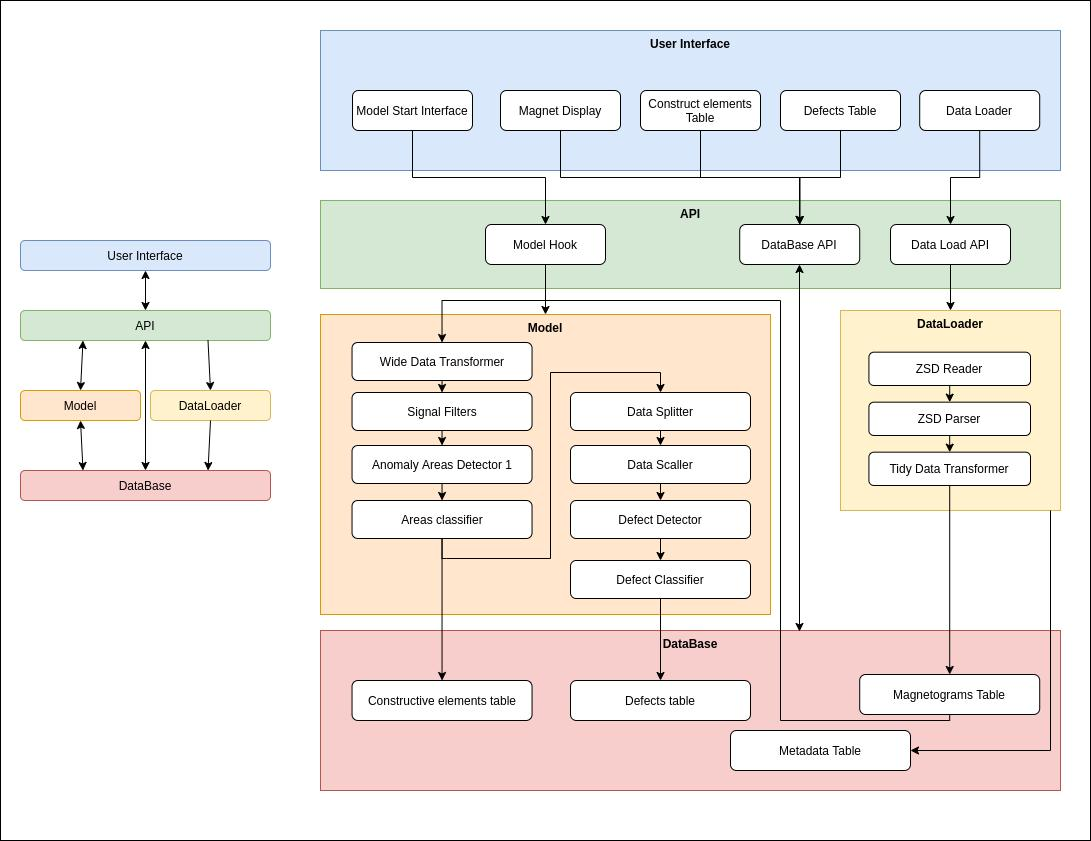
\includegraphics{images/image4.png}
    }
    
    \caption{
    \label{image3}
    Архитектура программного комплекса.}
    \end {center}
\end {figure}

\subsection{Структура и особенности данных}

Исходные данные зондов находились в бинарном формате. 
Для анализа и построения математической модели 
эти данные были расшифрованы и преобразованы в табличный формат “.csv” 
с помощью специально разработанного скрипта. 

Для каждой магнитограммы был следующий набор файлов: 
исходный файл магнитограммы в бинарном виде, преобразованный 
табличный файл магнитограммы “.csv” и экспертный отчет “.pdf” или “.doc”. 
В свою очередь в отчёте находилась информация об условиях съемки, 
а также давалась экспертная разметка магнитограммы с указанием конструктивных
элементов и дефектов (включая изображения соответствующих примеров). 
Всего в изначальном датасете было 36 магнитограмм, из которых 33 оказались 
уникальными (3 оставшиеся соответствовали повторному обследованию одних и 
тех же труб и не содержали дополнительной информации). Список, полученных после 
расшифровки магнитограмм параметров, приведён в Таблице 3. 

\begin{center}
\begin{longtable}{|p{2cm}|p{12cm}|p{2cm}|}
    \caption{Исходные данные}\\\hline
    Параметр & Описание & Единица \par измерения \\ \hline
    Tag & Начало новой записи данных (технический параметр) & - \\ \hline
    Size & Размер поля для записи данных (технический параметр) & - \\ \hline
    Time & Момент записи & мкс \\ \hline
    Dist & Значение дистанции & 10 мкм \\ \hline
    Index & Порядковый номер измерения & - \\ \hline
    Flags & Флаги сканирования (технический параметр)) & - \\ \hline
    Status X & Статус для блока из четырех датчиков, описывающий возможные ошибки в них: 0 – отсутствие ошибок; X – номер блока & - \\ \hline
    X.Y & Значение датчика Y из блока X; например: “1.3” & - \\ \hline
\end{longtable}
\end{center}

Термин “Технический параметр” означает, что данная переменная используется либо для расшифровки, 
либо для конверсии из исходного бинарного файла. Из приведённого списка для анализа магнитограмм 
наиболее важными факторами являются Dist и X.Y, так как именно они указывают на каком расстоянии 
находится дефект/шов/структурный элемент, и каким измеренным значениям он соответствует.

Первичный анализ данных, показал необходимость перепроверки и переразметки данных. Параметры, 
использованные для разметки сварных швов, дефектов и структурных элементов, приведены в Таблицах 4 и 5.

\begin{center}
    \begin{longtable}{|p{2cm}|p{12cm}|p{2cm}|}
        \caption{Параметры конструктивных элементов}\\\hline
        Параметр & Описание & Единица \par измерения \\ \hline
        id & Уникальный идентификатор конструктивного элемента – строка & - \\ \hline
        contructive type & Тип конструктивного элемента на основе отчетов & - \\ \hline
        start dist & Начало конструктивного элемента & 10 мкм \\ \hline
        end dist & Конец конструктивного элемента & 10 мкм \\ \hline
        wall width & Толщина стенки трубы на основе отчета & мм \\ \hline
    \end{longtable}
\end{center}

\begin{center}
    \begin{longtable}{|p{2cm}|p{12cm}|p{2cm}|}
        \caption{Параметры дефектов}\\\hline
        Параметр & Описание & Единица \par измерения \\ \hline
        id & Уникальный идентификатор дефекта – строка & - \\ \hline
        defect type & Тип дефекта на основе отчетов & - \\ \hline
        defect place & Местоположение дефекта: "Стенка трубы" или "Сварной шов"  & - \\ \hline
        defect depth & Глубина дефекта, на основе отчета  & \% \\ \hline
        start dist & Начало дефекта & 10 мкм \\ \hline
        end dist & Конец дефекта & 10 мкм \\ \hline
    \end{longtable}
\end{center}

После переразметки, в соответствующие папки магнитограмм были добавлены файлы конструктивных элементов 
$"construct\_element.csv"$ и файл разметки дефектов $"defect.csv"$.

При сопоставлении исходных данных магнитограмм с экспертной разметкой, приведённой в отчётах,
 было обнаружено расхождение длины пути зонда на расстояние вплоть до 150 см, что в свою очередь 
 привело к отличию координат дефектов и конструктивных элементов между датасетом и сопутствующим отчётом. 
 Предположительно, причиной этого расхождения является ошибка в ПО, используемом для генерации графиков к отчёту. 
 Для экспертного отчёта подобное расхождение является нежелательным, но не критичным, так как ремонт повреждённого 
 участка происходит не точечно, а в рамках целой секции трубы. В то же время, такое несоответствие между отчётом и 
 магнитограммой весьма негативно сказывается на точности математической модели, которая не может обучиться на противоречащих данных. 
 По этой причине силами сотрудников Дирекции Инновационного Развития была выполнена ручная проверка и переразметка
  датасета каждой магнитограммы (“.csv”), а обновлённые файлы были добавлены в соответствующие папки.

Важно заметить, что число записей (строк с показаниями датчиков) в магнитограмме зависят от пройденного 
зондом расстояния, которое может достигать 40 км. В представленном ниже датасете длина составляла 1.5-10 км. 
Участки свыше 10 км были исключены из рассмотрения в связи с трудоёмкостью уточнения изначальной разметки. 
В результате итоговый датасет составил 22 магнитограммы для анализа швов и 18 для анализа дефектов 
(некоторые трубы не имели дефектов согласно отчётам). Итоговый список магнитограмм для построения 
математической модели приведён в Таблице 6.

\begin{center}
    \begin{longtable}{|p{5cm}|p{5cm}|}
        \caption{Итоговый список магнитограмм}\\\hline
        Магнитограмма & Количество записей \\ \hline
        Магнитограмма №1 & 2125866 \\ \hline
        Магнитограмма №2 & 1470101 \\ \hline
        Магнитограмма №3 & 3815418 \\ \hline
        Магнитограмма №4 & 2482089 \\ \hline
        Магнитограмма №5 & 3761227 \\ \hline
        Магнитограмма №6 & 1072643 \\ \hline
        Магнитограмма №7 & 449613 \\ \hline
        Магнитограмма №8 & 711720 \\ \hline
        Магнитограмма №9 & 412681 \\ \hline
        Магнитограмма №10 & 1165283 \\ \hline
        Магнитограмма №11 & 3047114 \\ \hline
        Магнитограмма №12 & 575441 \\ \hline
        Магнитограмма №13 & 1498927\\ \hline
        Магнитограмма №14 & 683275 \\ \hline
        Магнитограмма №15 & 1108527 \\ \hline
        Магнитограмма №16 & 1630936 \\ \hline 
        Магнитограмма №17 & 338127 \\ \hline
        Магнитограмма №18 & 233018 \\ \hline
        Магнитограмма №19 & 291116 \\ \hline
        Магнитограмма №20 & 222167 \\ \hline
        Магнитограмма №21 & 860107 \\ \hline
        Магнитограмма №22 & 1772941 \\ \hline
    \end{longtable}
\end{center}

Для выявления особенностей данных были визуализированы данные для всех магнитограмм. 
Поскольку данные писались одновременно 64 независимыми датчиками, 
то для отображения графиков использовалось усреднённое значение по всем датчикам, 
записанное на данной координате (для сварных швов и структурных объектов). 
Для дефектов строились индивидуальные графики для каждого датчика. 
В итоге были зафиксированы следующие результаты (изображения ниже приводятся только для 
структурных элементов и сварных швов).

Определены паттерны конструктивного элемента "Сварной шов" и их средние показатели 
(ширина 5 сантиметров и высота 250 у.е.) (Рис. ~\ref{image4}).
\pagebreak

\begin{figure}[ht]
    \begin{center}
    \scalebox{0.35}{
       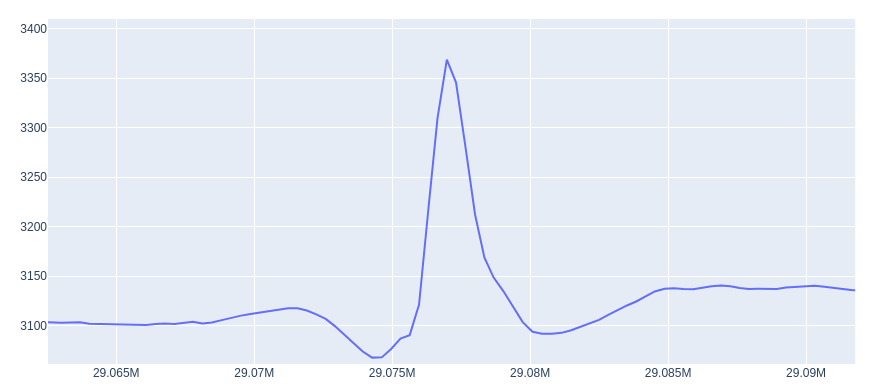
\includegraphics{images/image5.png}
    }
    
    \caption{
    \label{image4}
    Выделенный паттерн шва.}
    \end {center}
\end {figure}

\pagebreak

\begin{figure}[h!]
    \begin{minipage}[h]{0.9\linewidth}
    \center{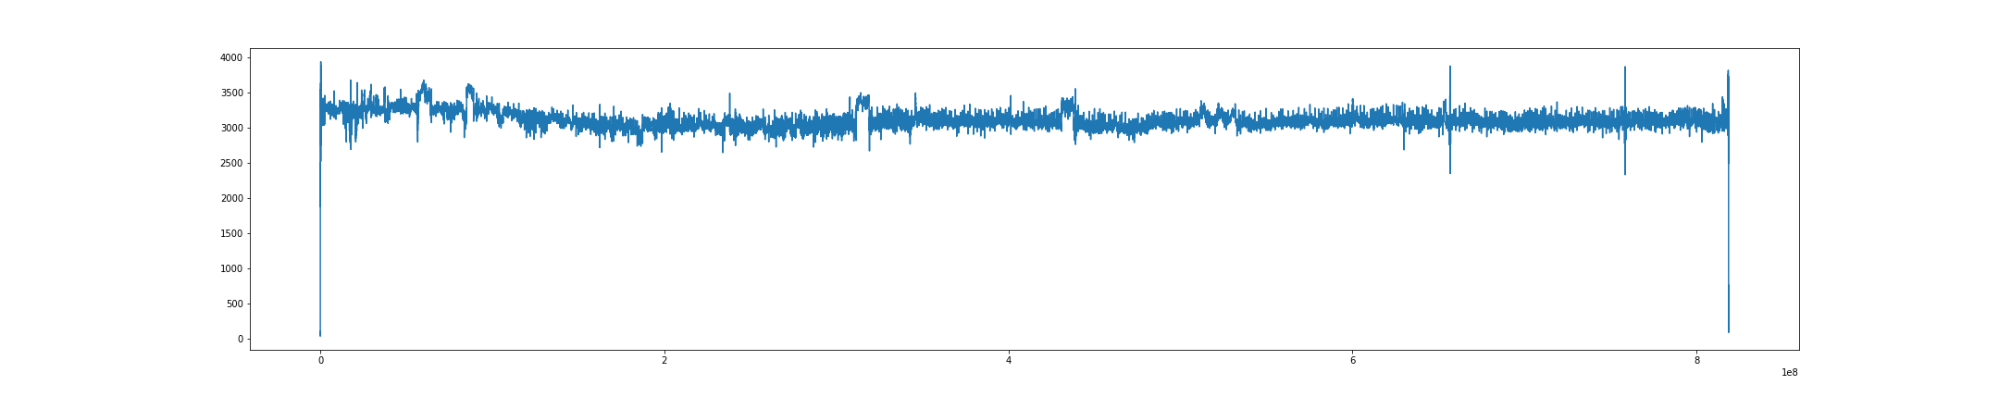
\includegraphics[width=1\linewidth]{images/image6.png}} Магнитограмма №1. \\
    \end{minipage}
    \vfill
    \begin{minipage}[h]{0.9\linewidth}
    \center{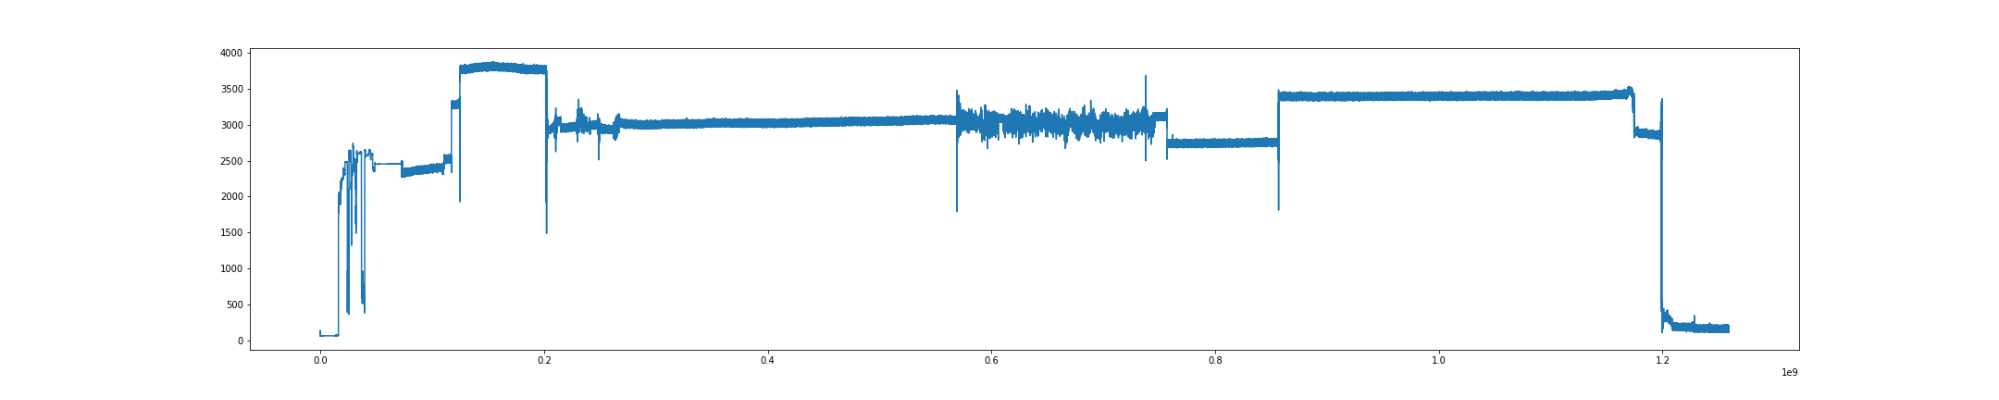
\includegraphics[width=1\linewidth]{images/image7.png}} Магнитограмма №3. \\
    \end{minipage}
    \vfill
    \begin{minipage}[h]{0.9\linewidth}
    \center{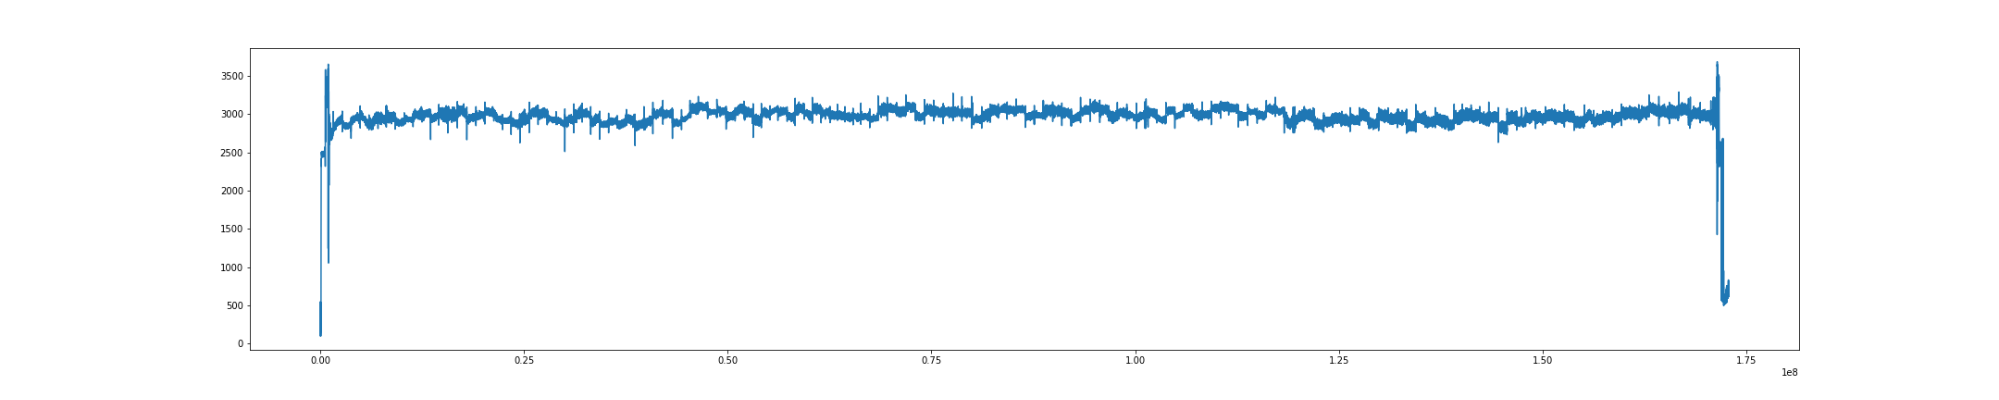
\includegraphics[width=1\linewidth]{images/image8.png}} Магнитограмма №9. \\
    \end{minipage}
    \vfill
    \begin{minipage}[h]{0.9\linewidth}
    \center{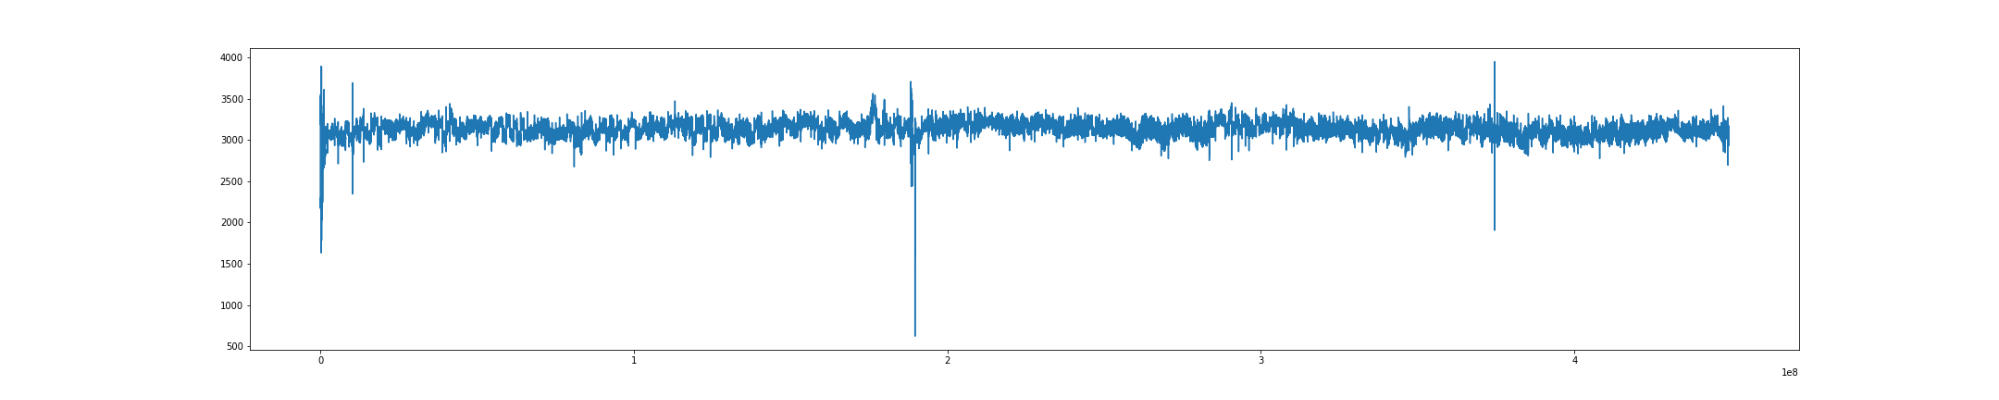
\includegraphics[width=1\linewidth]{images/image9.png}} Магнитограмма №10. \\
    \end{minipage}
    \vfill
    \begin{minipage}[h]{0.9\linewidth}
    \center{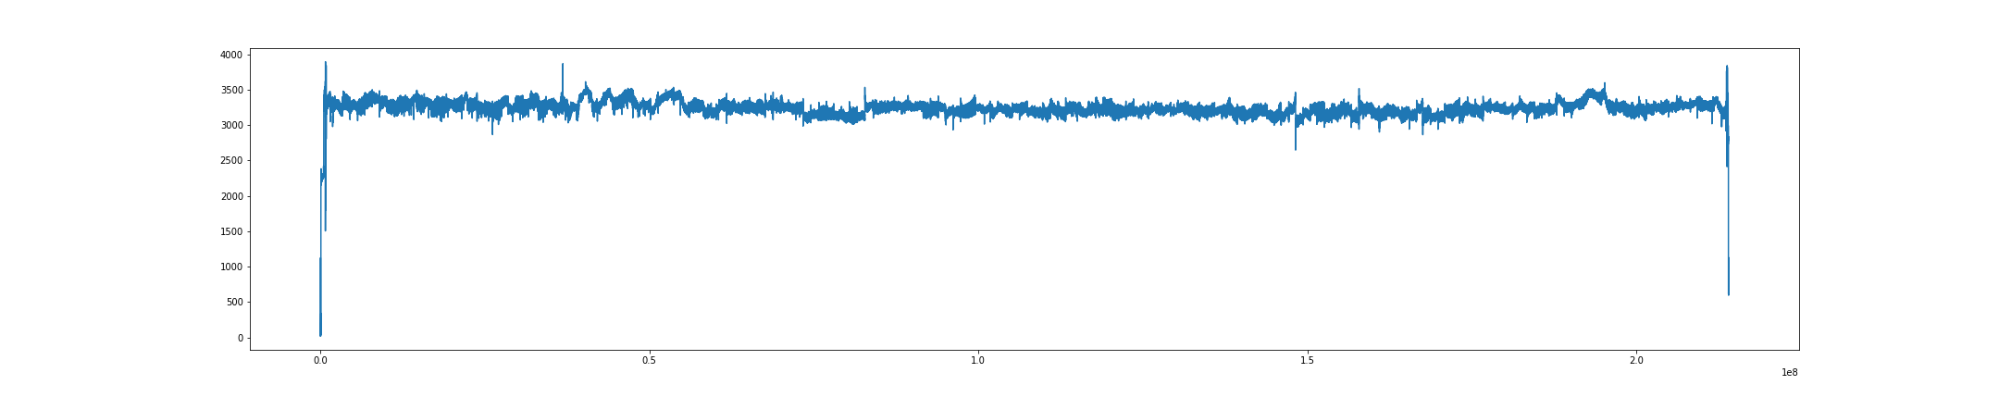
\includegraphics[width=1\linewidth]{images/image10.png}} Магнитограмма №12. \\
    \end{minipage}
    \vfill
    \begin{minipage}[h]{0.9\linewidth}
    \center{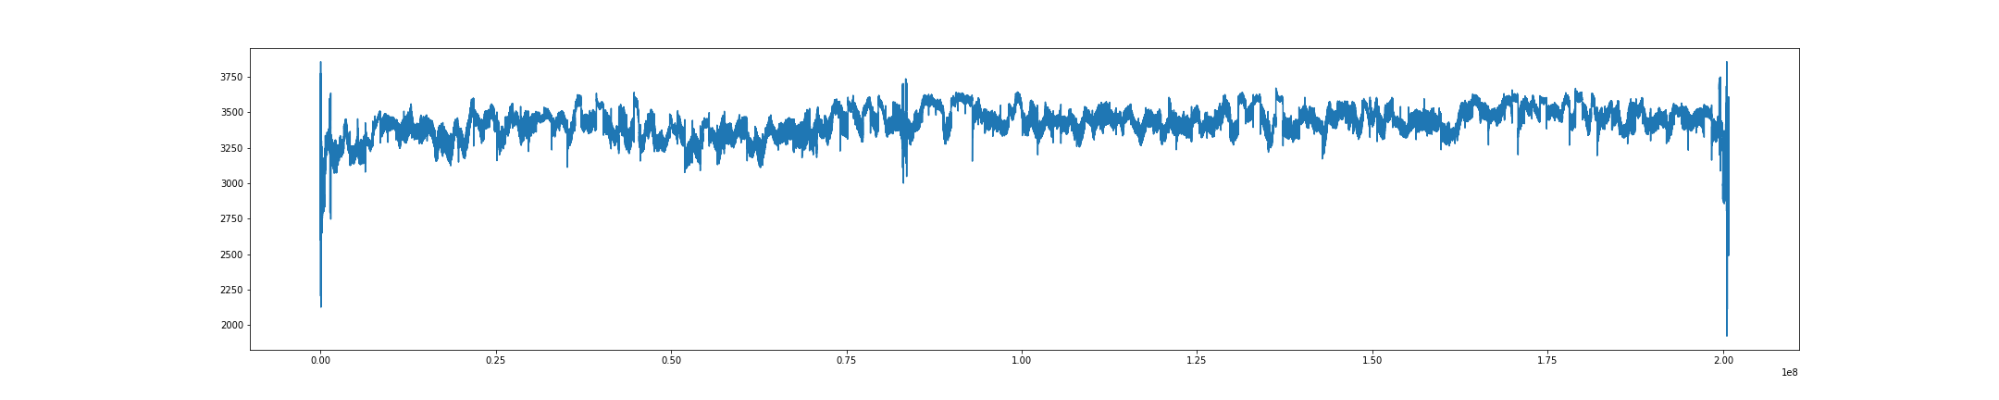
\includegraphics[width=1\linewidth]{images/image11.png}} Магнитограмма №14. \\
    \end{minipage}
    \caption{Магнитограммы с сильными шумами.}
    \label{image5}
\end{figure}

\pagebreak

\begin{figure}[h!]
    \begin{minipage}[h]{0.9\linewidth}
    \center{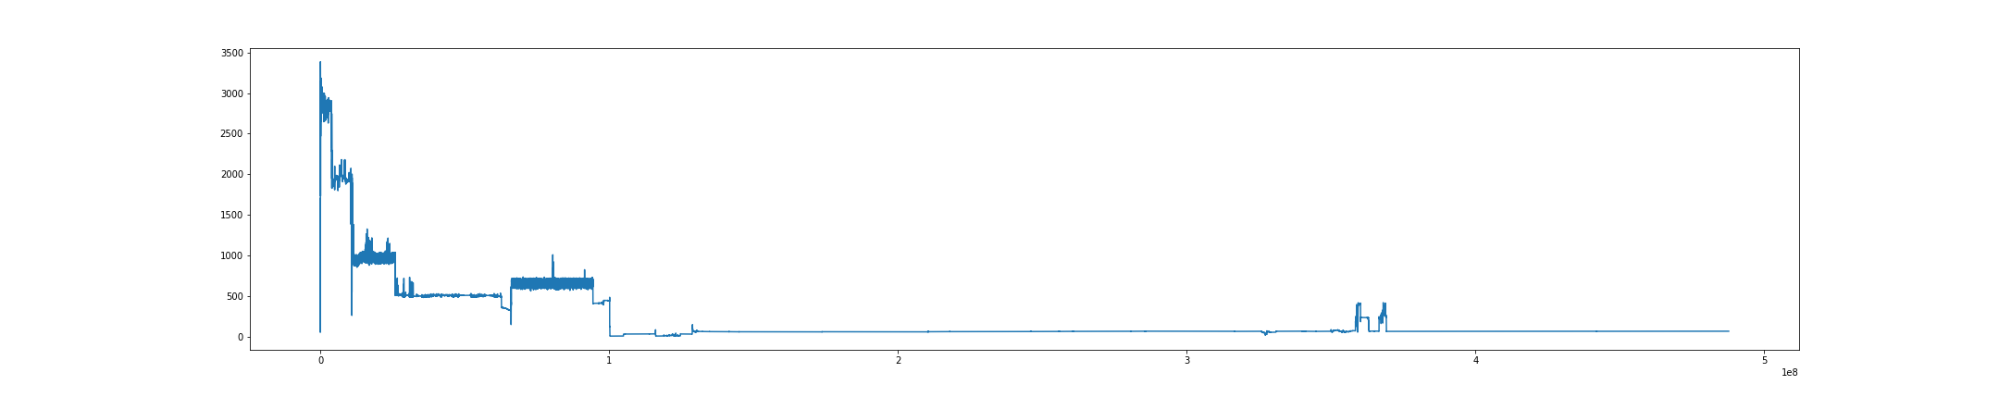
\includegraphics[width=1\linewidth]{images/image12.png}} Магнитограмма №2. \\
    \end{minipage}
    \vfill
    \begin{minipage}[h]{0.9\linewidth}
    \center{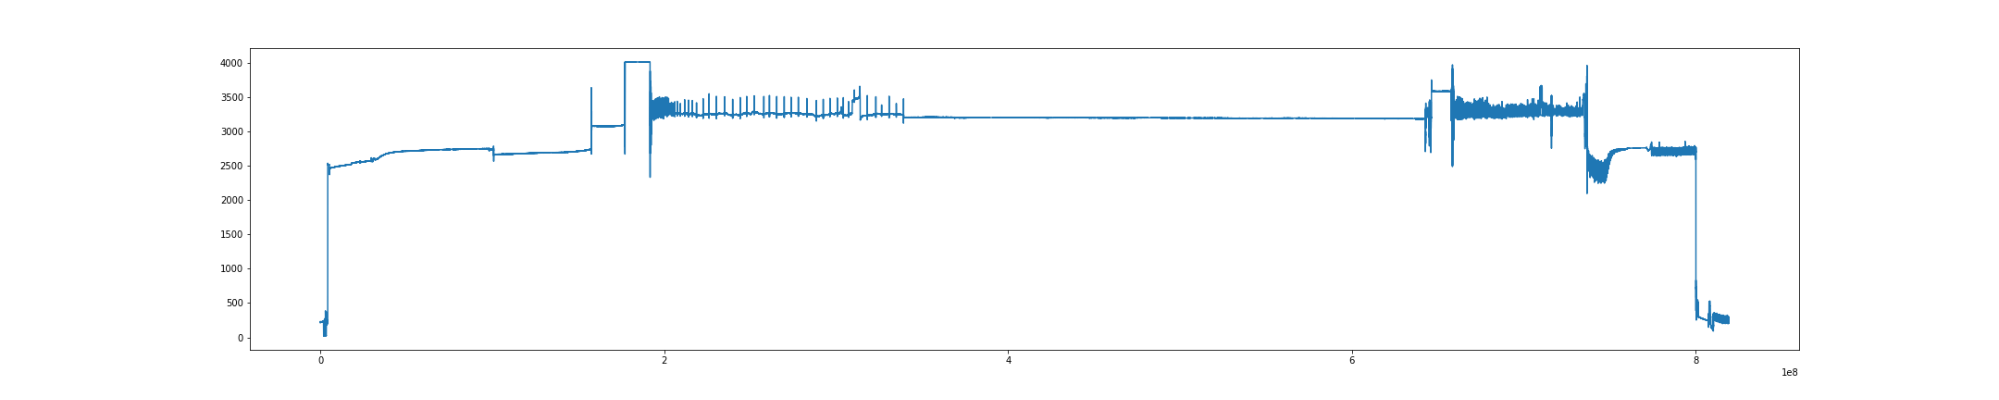
\includegraphics[width=1\linewidth]{images/image13.png}} Магнитограмма №4. \\
    \end{minipage}
    \vfill
    \begin{minipage}[h]{0.9\linewidth}
    \center{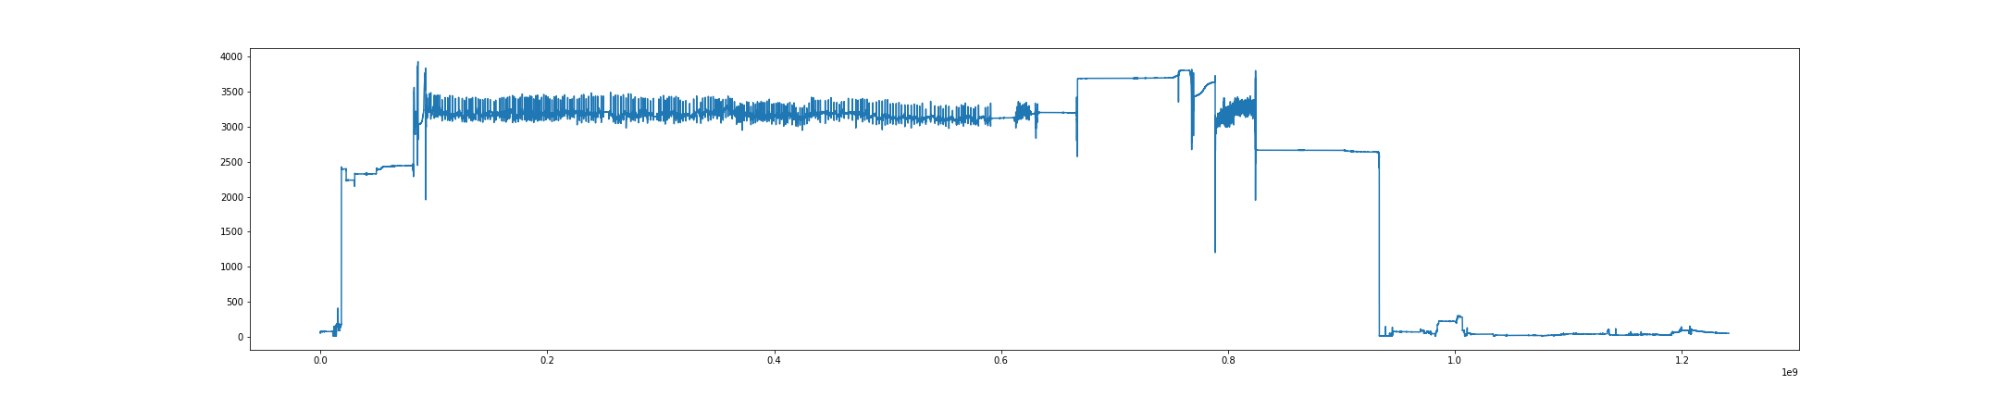
\includegraphics[width=1\linewidth]{images/image14.png}} Магнитограмма №5. \\
    \end{minipage}
    \vfill
    \begin{minipage}[h]{0.9\linewidth}
    \center{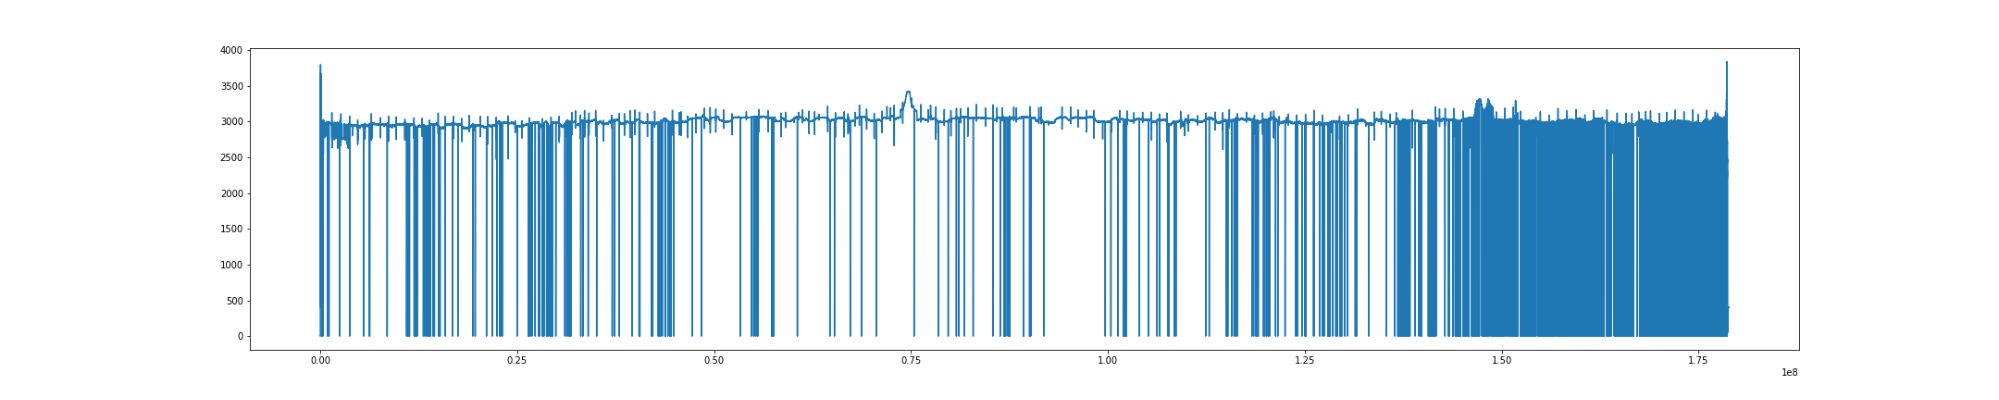
\includegraphics[width=1\linewidth]{images/image15.png}} Магнитограмма №7. \\
    \end{minipage}
    \vfill
    \begin{minipage}[h]{0.9\linewidth}
    \center{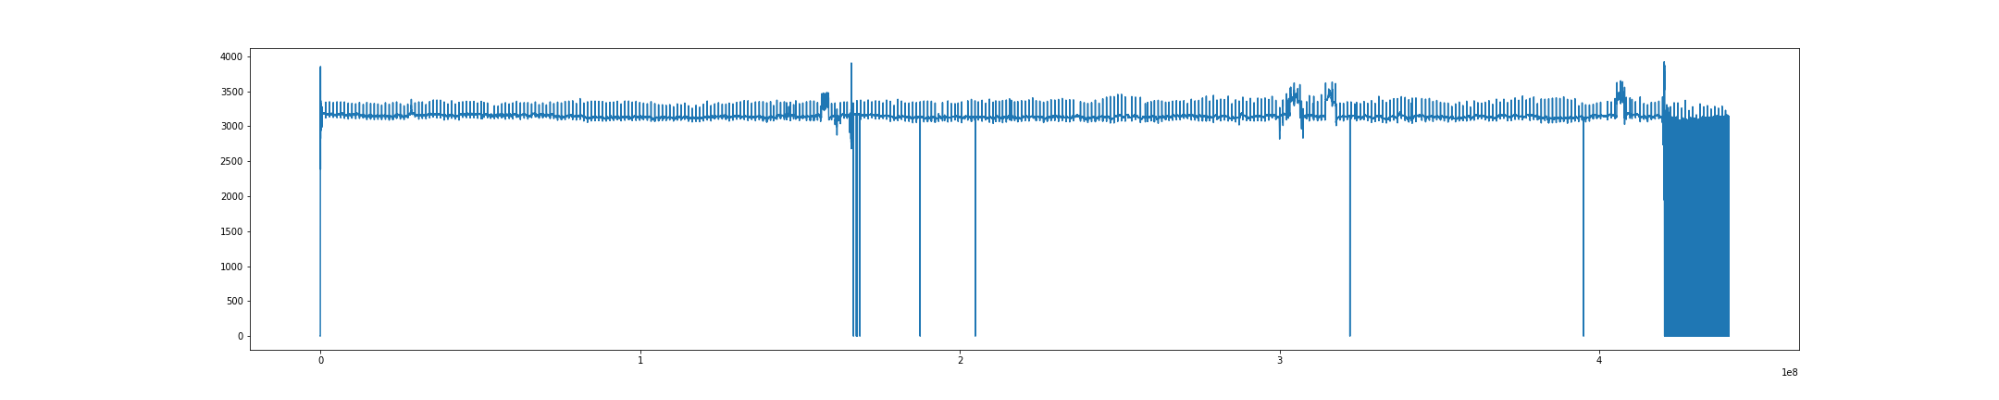
\includegraphics[width=1\linewidth]{images/image16.png}} Магнитограмма №15. \\
    \end{minipage}
    \vfill
    \begin{minipage}[h]{0.9\linewidth}
    \center{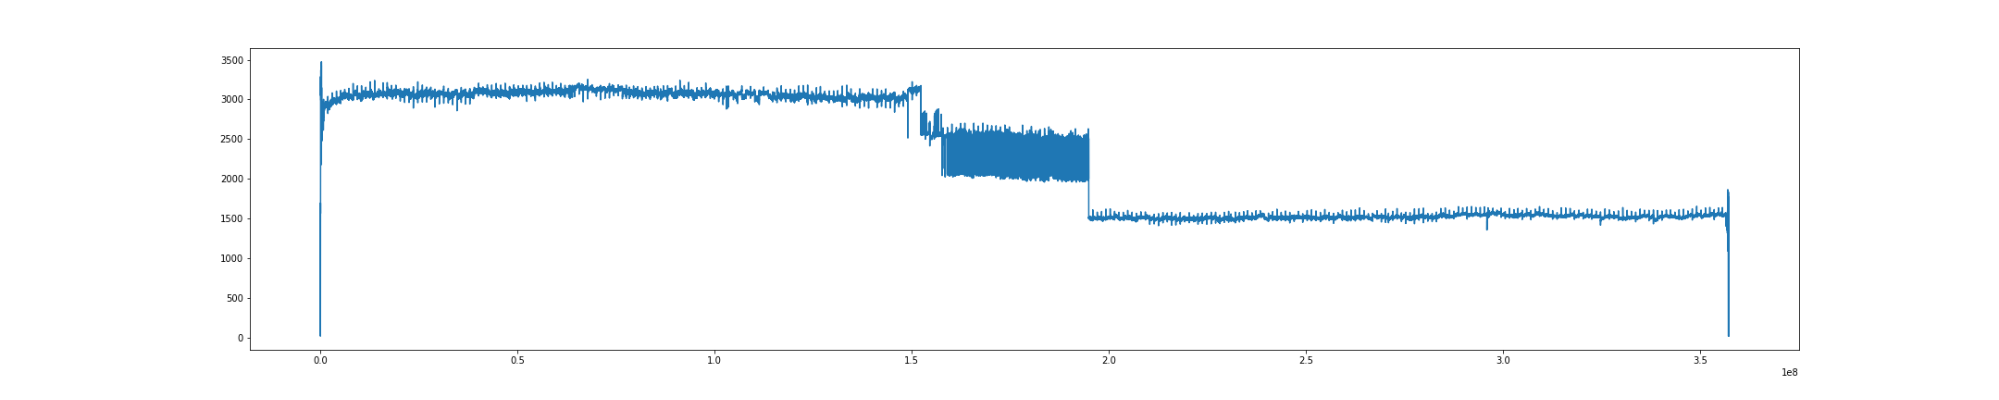
\includegraphics[width=1\linewidth]{images/image17.png}} Магнитограмма №16. \\
    \end{minipage}
    \caption{Магнитограммы с битыми или недостоверными данными.}
    \label{image6}
\end{figure}

Зашумлённые и "битые" магнитограммы также использовались для построения математической модели, но с заведомым ожиданием ухудшения качества детектирования на них.

\subsection{Процесс предобработки данных}

При анализе статусов блоков датчиков было замечено, что почти для половины магнитограмм 
датчики выдавали сообщения об ошибках. Поскольку эксперты всё же смогли разметить подобные "битые" 
данные, было принято решение не исключать проблемные магнитограммы и попробовать восстановить их двумя разными способами:

\begin{itemize}
    \item Анализ показаний статусов блоков датчиков. Данный подход оказался неудачным, ввиду того, что для некоторых магнитограмм количество ненулевых статусов соответствовало количеству выполненных измерений. Соответственно, во всей магнитограмме были отражены недостоверные данные (например, см магнитограмма №7 в Таблице 4).
    \item Проведение порогового анализа. На основе магнитограмм, визуально не имеющих битых данных, была рассчитана нижняя граница доверительного интервала показания датчиков. Определение "битых" / недостоверных данных проводилось с помощью рассчитанного порога: в среднем значения в магнитограмме по оси ординат колебались от 0 до 4000 у.е. (условных единиц); значения ниже 1000 у.е. экспертно были признаны недостоверными и заменены на арифметическое среднее по достоверным данным этой магнитограммы. Наглядные примеры различных "битых" и зашумлённых магнитограмм продемонстрированы на рисунках ~\ref{image5} и ~\ref{image6}.
\end{itemize}

Таким образом, метод порогового анализа позволил использовать для работы весь датасет, 
включая магнитограммы, состоящие только из "битых" данных. 

\subsection{Построение математической модели}

Для решения задач был выбран следующий подход:
\begin{itemize}
    \item Разработать аналитическое решение, способное определять области, схожие с паттерном сварного шва;
    \item Уточнить решение с помощью модели машинного обучения, обучив ее на подготовленной выборке;
    \item Провести разделение магнитограммы на секции по детектированным швам;
    \item Для каждой выделенной секции с помощью аналитического решения найти области, являющиеся локальными минимумами значений сигналов;
    \item Уточнить решение с помощью фильтрации и модели машинного обучения, обучив ее на подготовленной выборке.
\end{itemize}

\subsection{Выбор признаков}

Для обучения модели по детектированию швов на сформированном датасете в качестве признака 
было выбрано окно размером в 17 показаний на усредненном по всем датчикам сигнале: 
8 ближайших показаний левее заданной точки, показание на данной точке, 8 показаний правее. 
Размер окна был выбран эмпирическим образом после проведения экспериментов для максимизации значений 
метрик recall и precision.

Для обучения модели по детектированию дефектов на сформированном датасете в качестве признака 
было выбрано окно размером в 20 показаний на всех датчиках: 9 ближайших показаний левее заданной точки, 
показание для данной точки, 10 показаний правее. В результате выбора такого окна была получена матрица 
признаков размером n × 20, где n – количество датчиков. Для увеличения количества сэмплов с дефектами, 
производился циклический сдвиг полученной матрицы построчно: изначально строка с дефектом размещалась "внизу" 
матрицы, а затем на каждой итерации смещалась “вверх”, пока не оказывалась на первом месте. Подобная манипуляция 
была нужна чтобы проиллюстрировать принципиальную возможность нахождения дефекта в любом угловом секторе трубы. 
В противном случае, в процессе обучения модель могла бы решить, что дефекты всегда располагаются исключительно 
в определенном секторе, а похожие показания в других секторах – статистические выбросы. После подготовки всех 
семплов, полученные матрицы подверглась преобразованию в массив путем последовательной записи столбцов. 
Аналогично сварным швам, размер окна был выбран эмпирически, исходя из экспериментов для максимизации значения 
метрик recall и precision у модели машинного обучения.

\subsection{Решение по детектированию швов}

Аналитическое решение представляет собой алгоритм по поиску характерных пиков, явно выбивающихся из основного сигнала, 
и согласно картам разметки, соответствующих сварным швам. Основной проблемой такого подхода является наличие битых 
данных и сильная зашумленность некоторых магнитограмм. Для решения проблемы зашумленных данных были предприняты 
следующие шаги: 

\begin{itemize}
    \item Использование среднего значения показаний датчиков для анализа;
    \item Подсчет скользящего среднего с окном размером в 100 показаний и вычет его из сигнала;
    \item Подсчет скользящего среднего с окном размером в 2 показания и вычет его из сигнала. 
\end{itemize}

Также в ходе решения проблемы было рассмотрено применение фильтра Калмана и фильтра на основе вейвлет-преобразования. 
В финальную версию решения они не вошли, поскольку их применение к магнитограмме занимало значительно больше времени, 
чем весь остальной алгоритм аналитического решения. В частности, для одной магнитограммы длиной 1 км время работы 
фильтров составило:

\begin{itemize}
    \item Вейвлет фильтр – 123 минуты;
    \item Фильтр Калмана – 36 минут.
\end{itemize}

После применения описанных преобразований к усредненному сигналу, производился поиск пиков с помощью функции 
find peaks, реализованной в библиотеке SciPy. Для отсечения шумов использовались пороговые значения 
по относительной и абсолютной высоте пика. Для работы было определено пороговое значение, равное 1000.

Важно заметить, что данные фильтры использовались исключительно для аналитического решения, чтобы эффективнее 
выделять пики и находить их максимальные значения. При этом профиль самих пиков искажался, что делало невозможным 
их дальнейшее использование для обучения математической модели (разрабатываемая модель машинного обучения по-прежнему 
обучалась на зашумлённых данных, впрочем, теперь с уже точно заданными координатами пиков).

Далее после выделения областей интереса происходила фильтрация с помощью модели машинного обучения. 
Обучение модели проводилось на выделенных ранее признаках, соответсвующих двум классам: швам и полотну трубы. 
Баланс обучающей выборки был 1:1. 

\subsection{Решение по детектированию дефектов}

Для аналитического решения был выбран следующий подход:

\begin{itemize}
    \item Магнитограмма разбивалась на секции по швам;
    \item Для каждой секции производился поиск локальных минимумов значений сигналов датчиков;
    \item Производилась фильтрация выбранных минимумов по глубине.
\end{itemize}

Для поиска локальных минимумов производилась предобработка данных. Сначала данные интерполировались по 
дистанции для достижения сетки с равномерным шагом (т.е. пространственно измерения были равноудалены друг от друга). 
Также применялся гауссовский фильтр с целью уменьшения зашумленности. Минимумы искались с помощью функции find peaks, 
реализованной в SciPy. Данная функция применялась к среднему сигналу с каждого блока датчиков, умноженному на -1 
для отражения сигнала относительно оси абсцисс (Ох) на рисунках  ~\ref{image5} и ~\ref{image6}. Также производилась фильтрация пиков по их 
метапараметрам – ширине и относительной высоте. Для каждого пика сохранялись данные об абсолютной и относительной 
высоте, ширине, координатах левой и правой границ пика. Также производился подсчет процента глубины дефекта от общего 
сигнала. Наконец, для фильтрации дефектов применялся пороговый фильтр по проценту глубины потери металла.

После выбора зон возможных дефектов, производилось уточнение с помощью модели машинного обучения. Её обучение 
проводилось подобным образом, как описано в пункте выше.




\pagebreak
\section{Проведение эксперимента}

\subsection{Постановка эксперимента}

Для валидации алгоритмов по детектированию швов и дефектов было поставлено 7 экспериментов:
\begin{itemize}
    \item Валидация аналитического решения по детектированию швов
    \item Валидация бинарного классификатора для швов на подготовленном датасете
    \item Валидация алгоритма по детектированию швов
    \item Валидация аналитического решения по детектированию дефектов
    \item Валидация бинарного классификатора для швов на подготовленном датасете
    \item Валидация алгоритма по детектированию швов
    \item Тестирование алгоритмов на тестовой магнитограмме
\end{itemize}

Для валидации аналитических решений использовался весь набор магнитограмм. 
На его основе проводилась кросс-валидация - цикл оценки решения. На каждой 
итерации цикла выбиралась одна магнитограмма для разметки, а на основе оставшихся 
производилось обучение модели. После получения разметки она сопоставляется с разметкой 
экспертов и рассчитывались метрики. аналогичный подход использовался для валидации 
полных решений по детектированию швов и дефектов. Проверка бинарных классификаторов 
проводилась на основе заранее составленных  на основе экспертной разметки обучающих 
выборок для каждой из магнитограмм. Проверка также представляла собой процесс кросс-валидации. 
На каждой итерации выбиралась одна из выборок в качестве тестовой, а на остальных проводилось 
обучение алгоритма. Далее проводилась оценка модели на тестовой магнитограмме по заданным метрикам.

Помимо данных используемых для исследований, была выделена отдельная тестовая магнитограмма без 
разметки, которую требовалось интерпретировать, то есть предоставить информацию о расположении  
швов и дефектов. В дальнейшем полученная разметка сопоставлялась с трубными журналами.

\subsection{Результаты экспериментов}

Ниже представлены результаты проведенных экспериментов в виде таблиц с результатами кросс-валидации.

\begin{center}
    \begin{longtable}{|p{5cm}|p{3cm}|p{3cm}|}
        \caption{Метрики для аналитического решения по детектированию швов}\\\hline
        Магнитограмма & recall & precision \\ \hline
        Магнитограмма №1 & 0.914 & 0.297 \\ \hline
        Магнитограмма №2 & 0.889 & 0.002 \\ \hline
        Магнитограмма №3 & 0.821 & 0.013 \\ \hline
        Магнитограмма №4 & 0.951 & 0.355 \\ \hline
        Магнитограмма №5 & 0.986 & 0.636 \\ \hline
        Магнитограмма №6 & 0.953 & 0.677 \\ \hline
        Магнитограмма №7 & 0.939 & 0.173 \\ \hline
        Магнитограмма №8 & 0.963 & 0.225 \\ \hline
        Магнитограмма №9 & 0.951 & 0.172 \\ \hline
        Магнитограмма №10 & 0.813 & 0.12 \\ \hline
        Магнитограмма №11 & 0.955 & 0.717 \\ \hline
        Магнитограмма №12 & 0.738 & 0.101 \\ \hline
        Магнитограмма №13 & 0.929 & 0.315 \\ \hline
        Магнитограмма №14 & 0.714 & 0.164 \\ \hline
        Магнитограмма №15 & 0.972 & 0.433 \\ \hline
        Магнитограмма №16 & 0.979 & 0.774 \\ \hline
        Магнитограмма №17 & 0.945 & 0.448 \\ \hline
        Магнитограмма №18 & 0.885 & 0.327 \\ \hline
        Магнитограмма №19 & 0.988 & 0.756 \\ \hline
        Магнитограмма №20 & 0.934 & 0.337 \\ \hline
        Магнитограмма №21 & 0.962 & 0.852 \\ \hline
        Магнитограмма №22 & 0.964 & 0.705 \\ \hline
        Среднее & 0.91568 & 0.39086 \\ \hline
    \end{longtable}
\end{center}

Как видно из расчётов в таблице 7, аналитическая модель обладает высоким параметром recall (0.714-0.988, среднее 0.91568), но также достаточно низким precision (0.002-0.705, среднее 0.39086). 
Такой разброс precision продемонстрировал необходимость уточнения решения.

\begin{center}
    \begin{longtable}{|p{5cm}|p{3cm}|p{3cm}|}
        \caption{Кросс-валидация на Random Forest Classifier на швах}\\\hline
        Магнитограмма & recall & precision \\ \hline
        Магнитограмма №1 & 0.876747 & 0.949106 \\ \hline
        Магнитограмма №2 & 0.444444 & 0.8 \\ \hline
        Магнитограмма №3 & 0.934959 & 0.787671 \\ \hline
        Магнитограмма №4 & 0.896341 & 0.97351 \\ \hline
        Магнитограмма №5 & 0.969388 & 0.996503 \\ \hline
        Магнитограмма №6 & 0.994083 & 0.973913 \\ \hline
        Магнитограмма №7 & 0.807107 & 0.969512 \\ \hline
        Магнитограмма №8 & 0.950617 & 0.888462 \\ \hline
        Магнитограмма №9 & 0.993827 & 0.899441 \\ \hline
        Магнитограмма №10 & 0.972906 & 0.833333 \\ \hline
        Магнитограмма №11 & 0.988839 & 0.977925 \\ \hline
        Магнитограмма №12 & 0.907692 & 0.907692 \\ \hline
        Магнитограмма №13 & 0.855457 & 0.870871 \\ \hline
        Магнитограмма №14 & 0.980583 & 0.971154 \\ \hline
        Магнитограмма №15 & 0.997245 & 1 \\ \hline
        Магнитограмма №16 & 1 & 1 \\ \hline
        Магнитограмма №17 & 0.912088 & 0.954023 \\ \hline
        Магнитограмма №18 & 0.948718 & 0.986667 \\ \hline
        Магнитограмма №19 & 1 & 1 \\ \hline
        Магнитограмма №20 & 0.934211 & 0.898734 \\ \hline
        Магнитограмма №21 & 0.981191 & 0.96904 \\ \hline
        Магнитограмма №22 & 0.978088 & 0.983968 \\ \hline
        Среднее & 0.923842 & 0.935978 \\ \hline
    \end{longtable}
\end{center}

По результатам эксперимента, можно сделать заключение о применимости Random Forest Classifier в качестве 
оптимизатора, так как минимальное значение precision составляет 0.78 для модели. К тому же сильное 
падение метрик фиксируется только на магнитограммах отнесенных к зашумленным магнитограммам или 
магнитограммам сбитыми данными.

\begin{center}
    \begin{longtable}{|p{5cm}|p{3cm}|p{3cm}|}
        \caption{Метрики для итогового решения по детектированию швов}\\\hline
        Магнитограмма & recall & precision \\ \hline
        Магнитограмма №1 & 0.85 & 0.69 \\ \hline
        Магнитограмма №2 & 0.71 & 0.31 \\ \hline
        Магнитограмма №3 & 0.67 & 0.70 \\ \hline
        Магнитограмма №4 & 0.84 & 0.71 \\ \hline
        Магнитограмма №5 & 0.89 & 0.99 \\ \hline
        Магнитограмма №6 & 0.90 & 0.98 \\ \hline
        Магнитограмма №7 & 0.80 & 0.99 \\ \hline
        Магнитограмма №8 & 0.92 & 0.54 \\ \hline
        Магнитограмма №9 & 0.93 & 0.44 \\ \hline
        Магнитограмма №10 & 0.81 & 0.26 \\ \hline
        Магнитограмма №11 & 0.96 & 0.82 \\ \hline
        Магнитограмма №12 & 0.73 & 0.57 \\ \hline
        Магнитограмма №13 & 0.74 & 0.72 \\ \hline
        Магнитограмма №14 & 0.64 & 0.93 \\ \hline
        Магнитограмма №15 & 0.97 & 0.86 \\ \hline
        Магнитограмма №16 & 0.96 & 0.97 \\ \hline
        Магнитограмма №17 & 0.86 & 0.80 \\ \hline
        Магнитограмма №18 & 0.86 & 0.76 \\ \hline
        Магнитограмма №19 & 0.99 & 0.94 \\ \hline
        Магнитограмма №20 & 0.90 & 0.96 \\ \hline
        Магнитограмма №21 & 0.96 & 0.98 \\ \hline
        Магнитограмма №22 & 0.96 & 0.97 \\ \hline
        Среднее & 0.856 & 0.767 \\ \hline
    \end{longtable}
\end{center}

В процессе оценки, гипотеза об ухудшении качества за счет добавления магнитограмм, отнесенных к магнитограммам 
с зашумленными или битыми данными, подтвердилась. Напротив, при рассмотрении магнитограмм, не имеющих аномалий 
в данных, можно говорить о довольно высоких показателях recall и precision (больше 75\%).

\begin{center}
    \begin{longtable}{|p{5cm}|p{3cm}|p{3cm}|p{3cm}|}
        \caption{Результаты аналитического решения по детектированию дефектов}\\\hline
        Магнитограмма & Найдено дефектов & Дефектов в разметке & Совпадений с разметкой \\ \hline
        Магнитограмма №5	& 133	& 16	& 2 \\ \hline
        Магнитограмма №6	& 23824	& 17	& 15 \\ \hline
        Магнитограмма №7	& 17665	& 11	& 9 \\ \hline
        Магнитограмма №8	& 5847	& 9	    & 3 \\ \hline
        Магнитограмма №9	& 852	& 130	& 15 \\ \hline
        Магнитограмма №10	& 20437	& 3	    & 3 \\ \hline
        Магнитограмма №11	& 56637	& 80	& 68 \\ \hline
        Магнитограмма №12	& 2664	& 14	& 2 \\ \hline
        Магнитограмма №13	& 62	& 31	& 2 \\ \hline
        Магнитограмма №13	& 16726	& 49	& 13 \\ \hline
        Магнитограмма №14	& 12581	& 21	& 18 \\ \hline
        Магнитограмма №15	& 30631	& 15	& 14 \\ \hline
        Магнитограмма №17	& 3163	& 22	& 15 \\ \hline
        Магнитограмма №18	& 339	& 5	    & 1 \\ \hline
        Магнитограмма №19	& 11283	& 21	& 17 \\ \hline
        Магнитограмма №20	& 1502	& 9	    & 3 \\ \hline
        Магнитограмма №21	& 24151	& 24	& 19 \\ \hline
        Магнитограмма №22	& 56332	& 216	& 173 \\ \hline
        Сумма	& 284829	& 693	& 392 \\ \hline
    \end{longtable}
\end{center}

Стоит отметить, что оценка данного решения по метрикам затруднена за счет того, 
что экспертная разметка не является полной (при детальном анализе часть дефектов оказалась 
пропущенной экспертами при их разметке).

\begin{center}
    \begin{longtable}{|p{5cm}|p{3cm}|p{3cm}|}
        \caption{Результаты аналитического решения по детектированию дефектов} \\ \hline
        Магнитограмма	& recall	& precision \\ \hline
        Магнитограмма №5	& 0.761719	& 0.884354 \\ \hline
        Магнитограмма №6	& 0.244485	& 0.820988 \\ \hline
        Магнитограмма №7	& 0.960227	& 0.522815 \\ \hline
        Магнитограмма №8	& 0.946181	& 0.582265 \\ \hline
        Магнитограмма №9	& 0.964063	& 0.526036 \\ \hline
        Магнитограмма №10	& 1	        & 0.75 \\ \hline
        Магнитограмма №11	& 0.551172	& 0.868041 \\ \hline
        Магнитограмма №12	& 0.975446	& 0.556688 \\ \hline
        Магнитограмма №13	& 0.669962	& 0.601833 \\ \hline
        Магнитограмма №14	& 0.924107	& 0.671351 \\ \hline
        Магнитограмма №15	& 0.15	    & 0.993103 \\ \hline
        Магнитограмма №16	& 0.143145	& 0.662005 \\ \hline
        Магнитограмма №17	& 0.892045	& 0.842953 \\ \hline
        Магнитограмма №18	& 0.43125	& 0.901961 \\ \hline
        Магнитограмма №19	& 0.320685	& 0.814745 \\ \hline
        Магнитограмма №20	& 0.883681	& 0.538055 \\ \hline
        Магнитограмма №21	& 0.427734	& 0.948052 \\ \hline
        Магнитограмма №22	& 0.630859	& 0.913959 \\ \hline
        Среднее	& 0.65982	& 0.74440 \\ \hline
    \end{longtable}
\end{center}

Данный эксперимент показывает, что на хороших магнитограммах результаты Random Forest Classifier 
высоки и применимы для уточнения аналитической модели. Но в тоже время на магнитогрммах низкого 
качества recall падает до 0.15.

\begin{center}
    \begin{longtable}{|p{5cm}|p{3cm}|p{3cm}|p{3cm}|}
        \caption{Результаты аналитического решения по детектированию дефектов}\\\hline
        Магнитограмма & Найдено дефектов & Дефектов в разметке & Совпадений с разметкой \\ \hline
        Магнитограмма №5	& 76	& 16	& 2 \\ \hline
        Магнитограмма №6	& 2123	& 17	& 15 \\ \hline
        Магнитограмма №7	& 2749	& 11  	& 9 \\ \hline
        Магнитограмма №8	& 484	& 9	    & 5 \\ \hline
        Магнитограмма №9	& 265	& 130	& 54 \\ \hline
        Магнитограмма №10	& 4206	& 3	    & 1 \\ \hline
        Магнитограмма №11	& 2992	& 80	& 56 \\ \hline
        Магнитограмма №12	& 216	& 14	& 3 \\ \hline
        Магнитограмма №13	& 45	& 31	& 0 \\ \hline
        Магнитограмма №13	& 886	& 49	& 10 \\ \hline
        Магнитограмма №14	& 1412	& 21	& 18 \\ \hline
        Магнитограмма №15	& 215	& 15	& 1 \\ \hline
        Магнитограмма №17	& 84	& 22	& 5 \\ \hline
        Магнитограмма №18	& 61	& 5	    & 3 \\ \hline
        Магнитограмма №19	& 284	& 21	& 15 \\ \hline
        Магнитограмма №20	& 102	& 9	    & 1 \\ \hline
        Магнитограмма №21	& 73	& 24	& 2 \\ \hline
        Магнитограмма №22	& 483	& 216	& 56 \\ \hline
        Сумма	& 16756	& 693	& 256 \\ \hline
    \end{longtable}
\end{center}

В результате применения модели машинного обучения, количество верно детектируемых дефектов сильно 
упало и составляет только третью часть замеченных дефектов. но при этом общее число детектируемых 
областей уменьшилось на порядок.

Наличие тестовой магнитограммы гарантировало невозможность переобучения модели на тестовой выборке 
и позволяло провести независимую верификацию качества разрабатываемой математической модели. 
Данная магнитограмма была успешно размечена алгоритмом и была выслана Заказчику для экспертной 
проверки. Всего на ней было обнаружено 481 сварных шва и 14 дефектов.

\subsection{Выводы}

По результатам экспериментов, можно сказать о высоком качестве работы решения по детектированию швов 
как на магнитограммах хорошего качества, так и на магнитограммах содержащих битые, недостоверные или 
зашумленные данные.

Решение по детектированию дефектов хорошо себя показывает на магнитограммах высокого качества, 
имеющих малое количество шумов.  Некорректная идентификация большого числа дефектов обусловлена 
тем, что на некоторых магнитограммах присутствуют многочисленные шумы, которые, как и дефекты, 
являются локальными минимумами и определяются алгоритмом как дефекты.


\pagebreak
\specialsection{Заключение}

В рамках проведенных работ были выполнены следующие этапы:

\begin{itemize}
    \item Разработано программное обеспечение для преобразования файлов формата “.zsd” к табличному формату “.csv”;
    \item Проведена корректировка экспертной разметки с целью уточнения дистанций дефектов и конструктивных элементов для 22 магнитограмм; 
    \item Реализован прототип цифрового продукта, производящий автоматическую разметку магнитограммы с дальнейшей возможностью её корректировки в ручном режиме;
    \item Разработаны две модели для детектирования сварных швов и дефектов; результаты качественной оценки решений зафиксированы в разделt 3.2; 
\end{itemize}

При дальнейшем развитие проекта и доработке решения следует обогатить выборку за счет добавления новых магнитограмм 
с экспертной разметкой. Так же для улучшения работы самого решения существуют следующие возможности:

\begin{itemize}
    \item Применить фильтрацию к данным;
    \item Провести более подробный анализ паттерна дефекта;
    \item Обсудить с экспертами выявленные аномальные ситуации (в том числе их возможную физическую природу);
    \item Исследовать применимость дополнительных дата-саенс подходов (бустинговые деревья в текущей постановке задачи, нейросети для обработки изображений и выявления на них паттернов швов/дефектов);
    \item Провести детальный подбор гиперпараметров для моделей;
    \item Добавить такие метапризнаки, как ширина, высота, глубина и т.п. для детектируемого объекта.
\end{itemize}
\pagebreak
% Библиография в cpsconf стиле
% Аргумент {1} ниже включает переопределенный стиль с выравниванием слева
\begin{thebibliography}{1}
\bibitem{j1} Алексеев, А. Точки инновационного роста /А. Алексеев // \flqq Сибирская нефть\frqq. – 2019. – №161. – С. 46-52.
\bibitem{s1} Официальный сайт ООО "ИТСК": сайт. – URL: http://it-sk.ru/products/ (дата обращения: 06.03.2020). – Текст: электронный.
\bibitem{j2} Никоноров, А. Двигатель инноваций / А.Никоноров // \flqq Сибирская нефть\frqq. – 2018. – №152. – С. 52-58.
\bibitem{a1} Шалай, В.В. Анализ технического состояния объектов линейной част магистральных Нефтепроводов, определение оптимальных способов поддержания объектов линейной части в нормативном состоянии / В.В. Шалай, М.М. Васильев, К.А. Шумаков // \flqq Омский научный вестник\frqq – Омск, 2004. – С. 196-199.
\bibitem{s2} Официальный сайт \frqq Baker Huges\flqq: сайт. – URL: https://www.bakerhughes.com/ (дата обращения: 06.03.2020). – Текст: электронный.
\bibitem{s3} Официальный сайт \frqq Интрон gk.c\flqq: сайт. – URL: https://www.intron.ru/ (дата обращения: 06.03.2020). – Текст: электронный.
\bibitem{s4} Парк приборов для провдения ВТД компании \frqq Транснефть\flqq: сайт. – URL: https://diascan.transneft.ru/klientam/vnytritrybnaya-diagnostika/park-vnytritrybnih-inspekcionnih-priborov/?preview=1 (дата обращения: 06.03.2020). – Текст: электронный.
\bibitem{a2} Закирзаков А.Г., Егоров А.Л. АНАЛИЗ СОСТОЯНИЯ СЕТИ МАГИСТРАЛЬНЫХ НЕФТЕПРОВОДОВ ТЮМЕНСКОЙ ОБЛАСТИ НА ОСНОВЕ СТАТИСТИЧЕСКИХ ДАННЫХ // Современные проблемы науки и образования. – 2015. – №1-1. – URL: http://www.science-education.ru/ru/article/view?id=18926 (дата обращения: 23.04.2020).
\bibitem{a3} Чистяков С.П. СЛУЧАЙНЫЕ ЛЕСА: ОБЗОР // Труды Карельского научного центра РАН – 2013. – №1. – С. 117-136.
\bibitem{a4} Geurts, P., Ernst, D., Wehenkel, L. Extremely randomizedtrees // Machine Learning. – 2006. – №63. –  p.3–42.
\bibitem{a5} Srivastava, D., L. Bhambhu  Data classification  using  support  vector  machine. // Journal of Theoretical and Applied Information Technology. – 2010. – №12(1). – p. 1-7.
\bibitem{a6} Chao-Ying J. P., Lee K. L., Ingersoll G. M. An Introduction to Logistic Regression Analysis and Reporting. // The Journal of Educational Research. – 2002. – №96(1). – p. 3-14.
\bibitem{a7} Cheng J., Wang M. Automated detection of sewer pipe defects in closed-circuit television images using deep learning techniques // Automation in Construction. – 2018. – №95. – p. 155-171.
\bibitem{a8} Велькер Н.Н., Бондаренко А.В., Вершинин А.С., Дашевский Ю.А. ПРИМЕНЕНИЕ НЕЙРОННЫХ СЕТЕЙ ДЛЯ РЕШЕНИЯ ОБРАТНОЙ ЗАДАЧИ ВНУТРИТРУБНОЙ МАГНИТНОЙ ДЕФЕКТОСКОПИИ МАГИСТРАЛЬНЫХ ТРУБОПРОВОДОВ // Интерэкспо Гео-Сибирь. – 2018. – URL: https://cyberleninka.ru/article/n/primenenie-neyronnyh-setey-dlya-resheniya-obratnoy-zadachi-vnutritrubnoy-magnitnoy-defektoskopii-magistralnyh-truboprovodov (дата обращения: 23.04.2020).
\bibitem{a9} Murtagh F. Multilayer perceptrons for classification and regression // Neurocomputing. – 1991. – №2. –  p.183-197.
\bibitem{a10} Indolia S., Goswami A. K., Mishra S.P., Asopa P. Conceptual Understanding of Convolutional Neural Network- A Deep Learning Approach // Procedia Computer Science. – 2018. – №132. –  p.679-688.
\bibitem{a11} Дегтярев, A.A. Элементы теории адаптивного расширенного фильтра Калмана / А. А. Дегтярев, Ш. Тайль – Препринты ИПМ им. М. В. Келдыша, 2003 – 36 с.
\bibitem{a12} Демаков Н.В., Кузовников А.В., Пашков А.Е., Анжина В.А.  ФИЛЬТРАЦИЯ СИГНАЛОВ С ПОМОЩЬЮ ВЕЙВЛЕТ-ПРЕОБРАЗОВАНИЯ // Сибирский журнал науки и технологий – 2008.  – С. 40-44.
\bibitem{s5} Официальный сайт документации Python: сайт. – URL: https://www.python.org/ (дата обращения: 023.04.2020). – Текст: электронный.
\bibitem{s6} Официальный сайт документации C++: сайт. – URL: https://en.cppreference.com/w (дата обращения: 023.04.2020). – Текст: электронный.
\bibitem{s7} Официальный сайт документации React: сайт. – URL: https://ru.reactjs.org/ (дата обращения: 023.04.2020). – Текст: электронный.
\bibitem{s8} Официальный сайт документации Sqlite3: сайт. – URL: [https://www.sqlite.org/index.html (дата обращения: 023.04.2020). – Текст: электронный.
\bibitem{s9} Официальный сайт документации Scikit-Learn: сайт. – URL: https://scikit-learn.org/ (дата обращения: 023.04.2020). – Текст: электронный.
\bibitem{s10} Официальный сайт документации Pandas: сайт. – URL: https://pandas.pydata.org/ (дата обращения: 023.04.2020). – Текст: электронный.
\bibitem{s11} Официальный сайт документации Scipy: сайт. – URL: https://www.scipy.org/ (дата обращения: 023.04.2020). – Текст: электронный.
\bibitem{s12} Официальный сайт документации Flask: сайт. – URL: https://flask.palletsprojects.com/en/1.1.x// (дата обращения: 023.04.2020). – Текст: электронный.

\end{thebibliography}
\end{document}